\chapter{Governing Equations}
\label{chap:governing}
This chapter introduces the  equations governing fluid flow.
These are shown in their compressible form in \Cref{sec:ns} and
a brief introduction to turbulence modelling is given in \Cref{sec:turb}.
\section{Conservation laws}
\label{sec:ns}
The dynamical behavior of any fluid is determined by the following physical conservation laws~\cite{blazek2015computational}:
\begin{enumerate}
    \item Conservation of mass
    \item Conservation of momentum
    \item Conservation of energy
\end{enumerate}
Given equations of state connecting the thermodynamic variables, these laws form a system of equations that is mathematically closed, i.e. it can theoretically be solved using methods from calculus (analytically) alone if suitable assumptions, initial, and boundary conditions are supplied. An analytic solution has yet to be found and is currently one of the seven Millenium Prize problems~\cite{carlson2006millennium}. On the other hand, it is possible to solve approximations to these equations using computers (numerically) by discretizing the equations. This area of study is called Computational Fluid Dynamics (CFD).

The conservation laws impose conditions on the rate of change of mass, momentum and energy per unit volume, and can be expressed mathematically in a three-dimensional Cartesian coordinate system as:
\begin{align}
    \pdiff{\rho}{t} + \nabla \cdot
        (\rho\vec{u}) &= 0 \label{eq:mass}
    \\
    \pdiff{\rho\vec{u}}{t} \nabla\cdot(\rho\vec{u}\otimes\vec{u}) &= -\nabla p
     + \nabla \cdot \tau
     + \vec{S}_{M}
     \label{eq:mom}
     \\
    \pdiff{(\rho E)}{t} + \nabla\cdot(\rho\vec{u}H) &=
      \nabla\cdot(\tau\cdot\vec{u}) + \nabla\cdot(k\nabla T)
         + S_E
     \label{eq:energy},
\end{align}
where $\rho$ is the density, $\vec{u}$ the velocity vector, $\tau$ is the viscous stress tensor, $p$ is the fluid pressure, $\otimes$ is the outer product operator, $E$ is the specific energy of a fluid, $H$ is the specific total enthalpy, $T$ is the temperature and $k$ is the thermal conductivity coefficient. Readers are referred to~\cite{munson2012fundamentals} for a thorough derivation of these equations.

Assuming the fluid is Newtonian, the stress tensor $\tau$ can be written as:
\begin{equation*}
    \tau_{ij} = \mu \left [
        \pdiff{u_i}{x_j} + \pdiff{u_j}{x_i}
    \right ]
    + \lambda \left [
        \pdiff{u_k}{x_k}
    \right ] \delta_{ij}.
\end{equation*}
where $mu$ is the dynamic viscosity, a material property, and the strain-rate tensor $S_{ij}$ is defined as:
\begin{equation*}
    S_{ij} = \frac{1}{2}\left(
        \pdiff{u_i}{x_j} + \pdiff{u_j}{x_i}
    \right).
\end{equation*}
The specific energy is defined as:
\begin{equation*}
    E = i + \frac{1}{2}(u^2 + v^2 + w^2),
\end{equation*}
where $i$ is the internal thermal energy.
The specific total enthalpy and specific energy are related by the following:
\begin{equation*}
    H = E + \frac{p}{\rho}.
\end{equation*}

\Cref{eq:mass,eq:mom,eq:energy} form an under-determined system of five equations with seven unknowns: density, three components of velocity, pressure, temperature and specific energy. Equations of state are necessary to close the system. If the fluid is assumed to be a perfect gas, which is the case in most aerodynamic problems and all problems in this work, the following equations can be used:
\begin{align}
    p &= \rho R T \label{eq:state1}\\
    i &= c_v T \label{eq:state2},
\end{align}
where $R$ is the specific gas constant and $c_v$ is the specific heat at constant volume -- both are material properties.
% The conservation laws are expressed mathematically in the following section. It should be noted that the equations are based on the assumption that the fluid is a continuum, and therefore can be treated as a continuous substance, as opposed to discrete particles. Consequently, a mathematical abstraction called a \textit{control volume} is employed, which is the smallest possible element of fluid whose macroscopic properties, such as density and pressure, are not influenced by the individual molecules it is realistically comprised of.

%\subsection{Conservation of mass}
%The mass conservation equation requires that mass neither be created nor destroyed. The mass balance for a fluid element requires that the time rate of change of mass per unit volume plus the net flow rate of mass per unit volume be equal to zero. This statement can be expressed mathematically in a three-dimensional Cartesian coordinate system as:
% \begin{equation*}
%     \text{Rate of change of mass per unit volume}
%     = \pdiff{\rho}{t} +
%         \pdiff{(\rho u)}{x} +
%         \pdiff{(\rho v)}{y} +
%         \pdiff{(\rho w)}{z}
%     = 0
% \end{equation*}
% where $\rho$ is the fluid density and $u$, $v$ and $w$ are the velocity components in the $x$, $y$ and $z$ directions respectively. The above can also be written in vector notation:
% \begin{equation}
%     \pdiff{\rho}{t} + \nabla \cdot (\rho \vec{u}) = 0 \label{eq:mass}
% \end{equation}
% where $\vec{u}$ is the velocity vector.

% Similarly to the law of conservation of mass, the remaining conservation laws impose constraints on the rate of change of given properties. Let $\phi$ be an arbitrary conserved quantity per unit mass, its rate of change per unit volume can be written as:
% \begin{equation*}
%     \Dphi{\phi}
% \end{equation*}
% which is merely a generalization of~\Cref{eq:mass}. The second term is commonly referred to as the convective or advective term, since it is responsible for the transport of $\phi$ by the ordered motion of the flow.
% %
% \subsection{Conservation of momentum}
% %
% The law of conservation of momentum is obtained from Newton's second law, which requires that the rate of change of momentum of a fluid element equals the sum of forces on said element. In three dimensions, this translates to three equations:
% \begin{align*}
%     \Dphi{u} = F_x \\
%     \Dphi{v} = F_y \\
%     \Dphi{w} = F_z
% \end{align*}
% Forces on a fluid element can be split between two distinct types~\cite{versteeg2007introduction}:
% \begin{itemize}
%     \item surface forces
%     \begin{itemize}
%         \item pressure forces
%         \item viscous forces
%         \item gravity forces
%     \end{itemize}
%     \item body forces
%     \begin{itemize}
%         \item centrifugal forces
%         \item Coriolis forces
%         \item electromagnetic forces
%     \end{itemize}
% \end{itemize}
% Body forces as well as gravity forces are commonly lumped in a single source term $S_M$ in textbooks, as will be done here. The momentum equations can be written in vector form as:
% \begin{equation}
%  \pdiff{\rho\vec{u}}{t} + \nabla\cdot(\rho\vec{u}\otimes\vec{u}) = -\nabla p
%     + \nabla \cdot \tau
%     + \vec{S}_{M}
%     \label{eq:mom}
% \end{equation}
% where $\tau$ is the viscous stress tensor, $p$ is the fluid pressure and $\otimes$ is the outer product operator. This set of three equations is referred to as the Navier-Stokes equations. The corresponding equation for the $i$th Cartesian component is given by:
% \begin{equation*}
%     \Dphi{u_i} = -\pdiff{p}{x_i}
%     + \nabla \cdot (\tau_{ij}\boldsymbol{i}_j)
%     + S_{Mi}
% \end{equation*}
% where $\boldsymbol{i}_j$ is the Cartesian unit vector in the direction of $x_j$ and summation is implied on repeated indices, as per Einstein notation.

% Assuming the fluid is Newtonian, i.e. components of $\tau$ are related linearly to the components of the rate of deformation tensor, and that the fluid is isotropic, the components of the viscous stress tensor can be defined as:
% \begin{equation*}
%     \tau_{ij} = \mu \left [
%         \pdiff{u_i}{x_j} + \pdiff{u_j}{x_i}
%     \right ]
%     + \lambda \left [
%         \pdiff{u_k}{x_k}
%     \right ] \delta_{ij}
% \end{equation*}
% The dynamic viscosity $\mu$ relates stresses to linear deformation and the second viscosity $\lambda$ relates stresses to the volumetric deformation. The effect of the latter is small in practice, however a good approximation is typically obtained by using $\lambda = -\frac{2}{3}\mu$~\cite{schlichting1979aerodynamics}. Consequently, the stress tensor is defined throughout the rest of this work as:
% \begin{equation*}
%     \tau_{ij} = 2\mu \left(S_{ij} - \frac{1}{3} \pdiff{u_k}{x_k}\delta_{ij} \right)
% \end{equation*}
% where the strain-rate tensor $S_{ij}$ is defined as:
% \begin{equation*}
%     S_{ij} = \frac{1}{2}\left(
%         \pdiff{u_i}{x_j} + \pdiff{u_j}{x_i}
%     \right)
% \end{equation*}
% \subsection{Conservation of energy}
% %
% Let $E$ be the specific energy of a fluid, which is defined as
% \begin{equation*}
%     E = i + \frac{1}{2}(u^2 + v^2 + w^2)
% \end{equation*}
% where $i$ is the internal thermal energy. Also let, $T$ be the fluid temperature and $k$ be the thermal conductivity.
% The law of conservation of energy requires that the rate of change of specific energy be equal to the sum of the following:
% \begin{itemize}
%     \item work done on the fluid element:
%         $-\nabla\cdot(p\vec{u})
%             + \nabla\cdot(\tau\cdot\vec{u})$
%     \item net rate of heat addition: $\nabla\cdot(k \nabla T)$
%     \item rate of change of specific energy due to sources: $S_E$
% \end{itemize}
% where $k$ is the coefficient of thermal conductivity.
% Let $h$ be the specific enthalpy and $H$ be the specific total enthalpy, defined as
% \begin{align*}
%     h &= i + p/\rho\\
%     H &= h + \frac{1}{2}(u^2 + v^2 + w^2) = E + p/\rho
% \end{align*}
% The law of conservation of energy can then be expressed as
% \begin{equation}
%     \pdiff{(\rho E)}{t} + \nabla\cdot(\rho\vec{u}H) =
%         \nabla\cdot(\tau\cdot\vec{u}) + \nabla\cdot(k\nabla T)
%         + S_E
%     \label{eq:energy}
% \end{equation}
% It should be noted that~\Cref{eq:energy} introduces two new unknowns: the internal energy $i$ and the temperature $T$.

% When using air as the fluid, the thermal conductivity coefficient $k$ is commonly written as:
% \begin{equation*}
%     k = c_p\frac{\mu}{\Pran}
% \end{equation*}
% where $c_p$ is the specific heat at constant pressure and $\Pran$ is a dimensionless quantity called the Prandtl number. For air, the Prandtl number is equal to a constant 0.72.
% %
% \subsection{Equations of state}
% %
% The laws of conservation of mass (\Cref{eq:mass}), conservation of momentum (\Cref{eq:mom}) and conservation of energy (\Cref{eq:energy}) form a system of five partial differential equations (PDEs). Variables appearing in this system can be split between three different categories:
% \begin{enumerate}
%     \item Independent variables: $x$, $y$, $z$ and $t$
%     \item Dependent variables: $\rho$, $p$, $T$, $i$ and the velocity components $u$, $v$ and $w$
%     \item Material properties: $k$ and $\mu$
% \end{enumerate}
% All dependent variables are functions of all four independent variables. Solving for the dependent variables over a given problem domain is the ultimate goal of CFD, i.e. they are the unknowns of the problem. Whether the equations of state are necessary or not depends on the whether the flow is compressible or incompressible. If the fluid is a liquid or if the gas is flowing at low speeds, fluid density is essentially constant and the flow is deemed incompressible. In compressible flow, however, there are seven unknowns. With merely five independent equations, this is an under-determined system. The role of the equations of state is to close the system, in this case by providing two additional equations.

% Among the dependent variables are four so-called \textit{thermodynamic} variables: $\rho$, $p$, $T$ and $i$ (all but velocity). Linkage of these variables is obtained through the assumption of thermodynamic equilibrium, which is a safe enough assumption for most CFD problems~\cite{versteeg2007introduction}. The state of a substance in such an equilibrium can be fully described from just two state variables. The remaining variables are linked to the other two through equations of state.

% If the fluid is assumed to be a perfect gas, which is the case in most aerodynamic problems and all problems considered in this work, the following equations can be used:
% \begin{align}
%     p &= \rho R T \label{eq:state1}\\
%     i &= c_v T \label{eq:state2}
% \end{align}
% where $R$ is the specific gas constant and $c_v$ is the specific heat at constant volume -- both are material properties.
% %
%\subsection{Boundary conditions}
%
Finally, any problem definition in CFD requires specification of conditions at boundaries of the physical domain. There currently exists a wide range of available boundary conditions in the literature as well as commercial software. It is the user's responsibility to apply boundary conditions that would most accurately reflect the real behavior of the flow. In the scope of this work specifically, different CFD codes offer different choices of boundary conditions. For this reason, boundary conditions are discussed in the sections pertaining to the different flow solver implementations.
%
%
\section{Turbulence modelling}
\label{sec:turb}
%
\Cref{sec:ns} introduced the governing equations of the time-dependent three-dimensional fluid flow of a compressible Newtonian fluid. In theory, this set of equations can be solved numerically, provided initial and boundary conditions. This is what is called Direct Numerical Simulation (DNS). DNS for turbulent flows requires that all turbulent effects, which occur at very small temporal and spatial scales, be resolved. Consequently, DNS demands an equally small mesh spacing as well as a small time step size. The smaller the mesh spacing and time step, the more costly the computation, making DNS near impossible even on modern supercomputers.
%
\subsection{Random nature of turbulence}
%
The Reynolds number $\Rey$ is a dimensionless quantity commonly used to characterize fluid flows and is mathematically expressed as:
\begin{equation*}
    \Rey = \frac{\rho U l}{\mu},
\end{equation*}
where $l$ is a characteristic length and $U$ the velocity. The Reynolds number is a measure of the ratio of inertial forces to viscous forces. At low Reynolds numbers, fluid particles may follow relatively straight lines and minimal mixing occurs. For instance, a flow composed of a heterogeneous mixture may remain heterogeneous. This flow regime is referred to as laminar flow.

On the other hand, flow at high Reynolds numbers is rather chaotic and random. Fluid particles no longer follow straight lines and mixing is significantly increased. A heterogeneous mixture will quickly become homogeneous if it can. Flow properties such as velocity vary randomly in time and space, even if boundary conditions are constant. This regime is called turbulent flow. It also happens that many flows in engineering are turbulent~\cite{versteeg2007introduction}, as are all cases mentioned in the present work.

Turbulent flows are easily identifiable by the presence of vortices, or eddies, in the flow. Such a phenomenon was observed and documented as far back as the 15th century, by none other than Leonardo Da Vinci. \Cref{fig:vinci} depicts his studies of vortices in turbulent fluid motion. The lower drawing in this figure shows the formation of eddies of various sizes that is typical of turbulent flows. These eddies typically manifest themselves in the vicinity of velocity gradients, such as in free shear flows or near solid boundaries. The physical reason for which DNS is so costly is that it must resolve the production and decay of eddies in order to accurately simulate the flow.

The number of mesh points $N$ required to resolve turbulent effects can be related to the Reynolds number by~\cite{wilcox1998turbulence}:
\begin{equation*}
    N = \Rey^{2.25}.
\end{equation*}
Hence, memory storage requirements and CPU time grow significantly with the Reynolds number. In addition, the time step size must be reduced such that a fluid particle moves only a fraction of the mesh spacing. Thus, computational costs involved in DNS are too large for even simple problems in the turbulent regime.

\begin{figure}
    \centering
    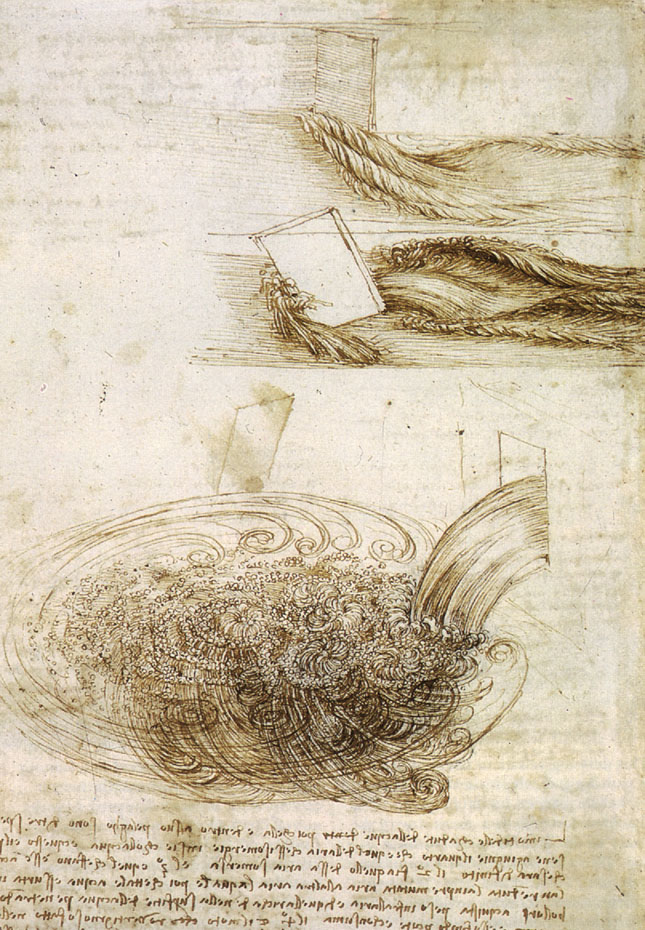
\includegraphics[width=0.3\textwidth]{figs/vinci}
    \caption{Studies of vortices in turbulent fluid motion by Leonardo da Vinci~\cite{wiki:vinci}.}
    \label{fig:vinci}
\end{figure}

Readers are referred to~\cite{pope2001turbulent,wilcox1998turbulence} for a more thorough discussion of turbulence.
%
\subsection{Favre-averaged Navier-Stokes equations}
%
For most engineering purposes it is unnecessary to resolve every detail of the turbulent fluctuations. In other words, merely solving for the so-called mean flow would be satisfactory. This would require a set of equations that is only concerned with the mean quantities of the flow. The most common, and probably simplest, way to obtain the mean flow equations is to write all conserved quantities appearing in the conservation equations as a sum of a fluctuating component and a mean component. Taking for instance an instantaneous conserved quantity $\phi$, one can write:
\begin{align*}
    \phi &= \ravg{\phi} + \phi'\\
    \ravg{\phi} &= \frac{1}{\text{T}} \int_{\text{T}}\phi(t)
        ~\text{d}t,
\end{align*}
where $\ravg{\phi}$ is the mean component, $\phi'$ is the fluctuating component, and $\text{T}$ is a time interval longer than the characteristic time scale of the turbulence. The mean component is then a time-averaged value, which is only relevant in statistically stationary (steady) flows. This work is only concerned with such flows. This technique is called a Reynolds decomposition.

To allow for compressibility effects, a mass weighted average must also be introduced. The Favre decomposition is defined as:
\begin{align*}
    \phi &= \favg{\phi} + \phi'' \\
    \favg{\phi} &= \frac{\overline{\rho\phi}}{\overline{\rho}}.
\end{align*}
It is important to note that $\ravg{\phi'} = 0$ but $\ravg{\phi''} \ne 0$.

In order to obtain a set of mean governing equations, a Reynolds decomposition for pressure and density and a Favre decomposition for velocity, internal energy and temperature is taken and substituted into the original (instantaneous) equation. Next, a time average of the resulting equations is taken.

It should be noted that the simpler Reynolds-averaged Navier-Stokes equations also exist but assume incompressible flow. Since the Favre-averaged equations are more general in that they do not rely on this assumption, as shown below.
%
\subsubsection{Conservation of mass}
%
Averaging of~\Cref{eq:mass} results in:
\begin{equation}
    \pdiff{\ravg{\rho}}{t}
        + \nabla\cdot \left(
            \ravg{\rho}\favg{\vec{u}}
        \right) = 0
    \label{eq:rmass}.
\end{equation}
This new equation is virtually identical to the original one, only with averaged values. Solving the original conservation of mass equation for instantaneous quantities is then no different than solving for the Favre-averaged quantities in the same time-averaged equation. As will be shown in the following sections, the same cannot be said of the remaining conservation laws.
%
\subsubsection{Conservation of momentum}
%
Averaging of~\Cref{eq:mom}, ignoring source terms, yields:
\begin{equation}
    \pdiff{\left(\ravg{\rho}\favg{\vec{u}}\right)}{t}
        + \nabla\cdot \left(
            \ravg{\rho}\favg{\vec{u}}\otimes\favg{\vec{u}}
        \right) =
        - \nabla\ravg{p}
        + \nabla\cdot\ravg{\tau}
        - \nabla\cdot
            \ravg{\rho \vec{u}''\otimes\vec{u}''}
    \label{eq:rmom}.
\end{equation}
This equation is also identical to~\Cref{eq:mom}, except for the additional term $\tau^T =  -\ravg{\rho \vec{u}''\otimes\vec{u}''}$. This term mathematically comes from the nonlinear convective term and represents the transfer of momentum due to turbulent fluctuations. Despite that, $\tau^T$ is known as the Reynolds-stress tensor. For clarity, the individual components of the Reynolds-stress tensor are defined as:
\begin{equation*}
    \tau^T_{ij} = \ravg{\rho u_i''u_j''}
\end{equation*}

Moreover, the turbulent kinetic energy $K$ is defined as the sum of the normal stresses (diagonal of the tensor) divided by density:
\begin{equation*}
    K = \frac{1}{2}\ravg{u_k''u_k''} = \frac{1}{2}\left[
        \ravg{(u'')^2)} + \ravg{(v'')^2)} + \ravg{(w'')^2)}
    \right]
\end{equation*}

Because the Reynolds stress tensor is symmetric, this adds a total of six unknowns to the three-dimensional momentum equations, leading to the \textit{turbulence closure problem}. In other words, the Favre-averaged, as well as Reynolds-averaged, conservation laws cannot be solved unless the Reynolds stresses are determined. A common solution to this problem is given in~\Cref{sec:bouss}.
%
\subsubsection{Conservation of energy}
%
Averaging of~\Cref{eq:energy}, again ignoring source terms, yields an equation with six additional terms. In practice, some of these terms are often ignored because they are assumed to be negligible~\cite{blazek2015computational}. After these assumptions are applied, the equation is written as:
\begin{align}
    \pdiff{\left(\ravg{\rho}\favg{E}\right)}{t}
    + \nabla\cdot\left(\ravg{\rho} \favg{\vec{u}} \favg{H}\right)
    =
    \nabla\cdot\left[
        \ravg{\tau}\cdot\favg{\vec{u}}
        + k\nabla\favg{T}
         -\tau^T\cdot\favg{\vec{u}}
         - \ravg{\rho \vec{u}'' h''}
    \right]
    \label{eq:renergy}
\end{align}
Moreover, the total energy and total enthalpy can be expressed as:
\begin{align*}
    \ravg{\rho}\favg{E} &= \ravg{\rho}\favg{e}
        + \frac{1}{2}\ravg{\rho}\favg{u_k}\favg{u_k} + K\\
    \ravg{\rho}\favg{H} &= \ravg{\rho}\favg{h}
        + \frac{1}{2}\ravg{\rho}\favg{u_k}\favg{u_k} + K
\end{align*}
%
An investigation of~\Cref{eq:renergy} reveals two additional terms as compared to~\Cref{eq:energy}. These are the last two terms on the right-hand side, and represent the work done by Reynolds stresses and turbulent transport of heat, respectively. In contrast, the first two terms on the right-hand side represent the work done by viscous stresses and diffusion of heat.

Averaging of the conservation of energy equation adds another three unknowns to the system, these are the components of the heat-flux vector $\ravg{\rho \vec{u}'' h''}$.
\subsection{Approximations to turbulent terms}
%
\label{sec:bouss}
The temporal averaging process detailed in the previous subsection introduces new terms to the system of equations. The challenge, which
has yet to be completely overcome even today, is to correctly
\textit{model} the additional turbulent terms $\tau^T$ and
$\ravg{\rho \vec{u}'' h''}$. This is done through a turbulence model.

In 1877, Boussinesq observed that the momentum transfer in a turbulent flow is dominated by the mixing caused by large energetic turbulent eddies~\cite{blazek2015computational}. The Boussinesq approximation then states that the turbulent stress is proportional to the mean strain rate, where the proportionality factor is the so-called eddy viscosity $\mu_T$. This can be written as:
\begin{equation}
    \tau^T_{ij} = 2\mu_T \left(
        \favg{S} - \frac{1}{3}\pdiff{u_k}{x_k}\delta_{ij}
    \right) - \frac{2}{3}\favg{\rho}K\delta_{ij}
    \label{eq:bouss}
\end{equation}
Whereas the dynamic viscosity is a property of the fluid, the eddy viscosity is, or should be, entirely a property of the flow. This is the reason why it is difficult to correctly approximate the term. Nonetheless, this has effectively removed five unknowns from the Favre-averaged conservation laws, since none of the other quantities in $\tau_T$ are new.

A Reynolds analogy can be used to model the turbulent heat flux as such:
\begin{equation}
    \ravg{\rho \vec{u}'' h''} = -c_p\frac{\mu_T}{\Pran_T}\nabla\favg{T}
\end{equation}
where $\Pran_T$ is the turbulent Prandtl number, which is assumed to be constant and is equal to 0.9 for air.

Now that both turbulent terms have been modelled, it is convenient to combine the turbulent and laminar components into \textit{effective} components:
\begin{align*}
    \mu_{\text{eff}} &= \mu + \mu_T\\
    k_{\text{eff}} &= c_p\left(
        \frac{\mu}{\Pran} + \frac{\mu_T}{\Pran_T}
    \right)
\end{align*}
The sum of viscous and Reynolds stresses can then be written as:
\begin{align*}
    \tau_{ij} + \tau_{ij}^T =
        \mu_{\text{eff}}\left(
            \pdiff{u_i}{x_j} + \pdiff{u_j}{x_i}
            - \frac{2}{3}\pdiff{u_k}{u_k}\delta_{ij}
        \right) - \frac{2}{3}\rho K \delta_{ij}
\end{align*}
It is then possible to rewrite the Favre-averaged Navier-Stokes equations, noting that the average symbols have been dropped, i.e. every quantity is effectively an averaged quantity.
\begin{align}
    \Dphi{} &= 0 \label{eq:fansmass}\\
    \pdiff{\rho \vec{u}}{t} + \nabla\cdot(\rho\vec{u}\otimes\vec{u}) &=
        -\nabla p + \nabla\cdot(\tau + \tau^T) \label{eq:fansmom}
    \\
    \pdiff{\rho E}{t} + \nabla\cdot (\rho \vec{u} H) &=
        \nabla\cdot \left[
            (\tau + \tau^T) \cdot \vec{u}
        \right]
        - \nabla\cdot\left(k_{\text{eff}}\nabla T\right) \label{eq:fansenergy}
\end{align}
Thus, only the specification of the eddy viscosity is needed in order to solve the Favre-averaged Navier-Stokes equations. It is crucial to remember that the eddy viscosity does not exist, it is nothing but a convenient mathematical invention whose purpose is to \emph{model} the production and decay of eddies in the flow.
%
\subsection{Law of the wall}
%
The total shear stress is the sum of viscous and Reynolds stresses. The Reynolds stresses being null at a wall, since $\vec{u} = 0$, the total shear stress at the wall $\tau_w$ is due entirely to the viscous contribution. It was found through experimentation and simulation that the Reynolds stresses tend to dominate as one moves away from the wall~\cite{pope2001turbulent}. In fact, the relative importance of both sources of stress can be determined through a non-dimensional wall distance $y^+$ defined by:
\begin{equation*}
    y^+ = \frac{u_\tau d}{\nu},
\end{equation*}
where $d$ is the distance to the nearest wall and $u_\tau$ is the friction velocity defined as:
\begin{equation*}
    u_\tau = \sqrt{\frac{\tau_w}\rho}.
\end{equation*}.
It is possible to identify the following layers in the near-wall flow based on the $y^+$ value:
\begin{description}
    \item[Viscous sublayer] ($y^+ < 5$): Viscous stresses dominate
    \item[Buffer layer] ($5 < y^+ < 30$): Neither stress dominates
    \item[Log-law layer] ($y^+ > 30$): Turbulent stresses dominate
\end{description}
Another quantity of interest is the non-dimensional velocity $u^+ = U/u_\tau$ where $U$ is the velocity parallel to the wall, which can be related to $y^+$ through a function $f_w(y^+)$. For fully turbulent flows, the function $f_w$ has been found to be universal and to vary depending on the layer as follows:
\begin{description}
    \item[Viscous sublayer]: $u^+ = y^+$
    \item[Log-law layer]: $u^+ = \frac{1}{\kappa} \ln y^+ + C^+$
\end{description}
where $\kappa \approx 0.41 $ is the Von Kármán constant and $C^+\approx5.0$ for a smooth wall~\cite{pope2001turbulent}. There is no clear relationship between $u^+$ and $y^+$ in the buffer layer, as the contributions to the shear stress are mixed.

In CFD packages that solve the averaged equations, it is recommended to have at least a few points within the viscous sublayer in order to resolve the flow correctly. Thus, in practice, the computation of $y^+$ is useful in determining whether the mesh requires refinement.
%
\subsection{Spalart-Allmaras model}
\label{sec:sa}
The Spalart-Allmaras model adds one partial differential equation for an artificial variable called the \textit{modified eddy viscosity}, identified by $\sa$. It is related to the eddy viscosity through a simple algebraic equation:
\begin{align*}
    \mu_T &= \rho \sa f_{v1}\\
    f_{v1} &= \frac{\chi^3}{\chi^3 + c_{v1}^3}\\
    \chi &= \frac{\sa}{\nu},
\end{align*}
where $\nu = \mu/\rho$ is the kinematic viscosity.

The modified eddy viscosity is governed by the following transport equation:
\begin{equation}
    \pdiff{\sa}{t} + \vec{u}\cdot(\nabla\sa) =
        c_{b1}(1 - f_{t2})\hat{S}\sa
        - \left[
            c_{w1}f_w - \frac{c_{b1}}{\kappa^2}f_{t2}
        \right] \left(
            \frac{\sa}{d}
        \right)^2
        + \frac{1}{\sigma}\nabla\cdot\left[ (\nu + \sa) \nabla\sa \right]
        + \frac{c_{b2}}{\sigma}\left(\nabla \sa\right)^2
        \label{eq:sa},
\end{equation}
where $d$ is the distance to the nearest solid wall. Additional definitions are given by:
\begin{align*}
    f_{t2} &= c_{t3} \text{exp}(-c_{t4}\chi^2)\\
    \hat{S} &= \Omega + \frac{\sa}{\kappa^2 d^2}f_{v2}, \quad
        f_{v2} = 1 - \frac{\chi}{1 + \chi f_{v1}}, \quad
        \Omega = \sqrt{2W_{ij}W_{ij}}, \quad
        W_{ij} = \frac{1}{2}\left(\pdiff{u_i}{x_j} + \pdiff{u_j}{x_i}\right)\\
    f_{w} &= g \left[
        \frac{1 + c_{w3}^6}{g^6 + c_{w3}^6}
    \right]^{1/6}, \quad
        g = r + c_{w2}(r^6 - r), \quad
        r = \text{min}\left[ \frac{\sa}{\hat{S}\kappa^2d^2}, 10 \right].
\end{align*}

The constants are:
\begin{gather*}
    c_{b1} = 0.1355, \quad \sigma = 2/3, \quad c_{b2} = 0.622, \quad \kappa = 0.41\\
    c_{w2} = 0.3, \quad c_{w3} = 2, \quad c_{v1} = 7.1, \quad c_{t3} = 1.2\\
    c_{t4} = 0.5, \quad c_{w1} = \frac{c_{b1}}{\kappa^2} + \frac{1 + c_{b2}}{\sigma}.
\end{gather*}
The boundary conditions are:
\begin{itemize}
    \item $\sa = 0$ at solid walls.
    \item $\sa = 3\nu_\infty$ to $5\nu_\infty$ in the far-field.
\end{itemize}
Comparison of \Cref{eq:sa} with the Navier-Stokes equations reveals some similarities. The left-hand side is comprised of the time rate of change of a quantity, in this case the modified eddy viscosity, and the advection of the stated quantity. The terms on the right-hand side represent the production, destruction, diffusion and anti-diffusion of $\sa$, respectively.

There exists several variants of the model, which are enumerated in~\cite{tmrsa}. A common variant involves neglecting the $f_{t2}$ term. Based on studies in~\cite{rumsey2007apparent}, use of this form makes little difference in the solution at reasonably high Reynolds numbers, provided that the far-field $\sa$ value is large enough. Other variants involve changes to the production term to account for rotation and curvature effects~\cite{shur2000turbulence,dacles1995numerical,dacles1999numerical}. Some other variants slightly alter the model so as to prevent values of $\sa$ from being negative

It should be emphasized that this is a model, as opposed to a mathematical expression of a law like the Navier-Stokes equations. Most turbulence models involve the calculation of the wall distance $d$, the accuracy of which can have a significant impact on the solution.

Finally, while some models involve the computation of the turbulent kinetic energy, the Spalart-Allmaras model does not. Thus, the last term in~\Cref{eq:bouss} involving $k$ is ignored. In practice, this term is small compared to the others, especially in non-supersonic flows~\cite{tmrsa}.

